%%%%%%%%%%%%%%%%%%%%%%%%%%%%%%%%%%%%%%%%%%%%%%%%%%%%%%%%%%%%%%%%%%%%%%%%%%%

\documentclass{standalone}

\usepackage{amsmath}
\usepackage{mathptmx}
\usepackage{pgfplots}
\usetikzlibrary{external}
\tikzexternalize{a-sin-b}
\pgfplotsset{compat=1.16}

%% IEEE uses Times Roman font, so we'll default to Times.
%% These three commands make up the entire times.sty package.
\renewcommand{\rmdefault}{ptm}
\renewcommand{\ttdefault}{pcr}
\normalfont\selectfont

\begin{document}

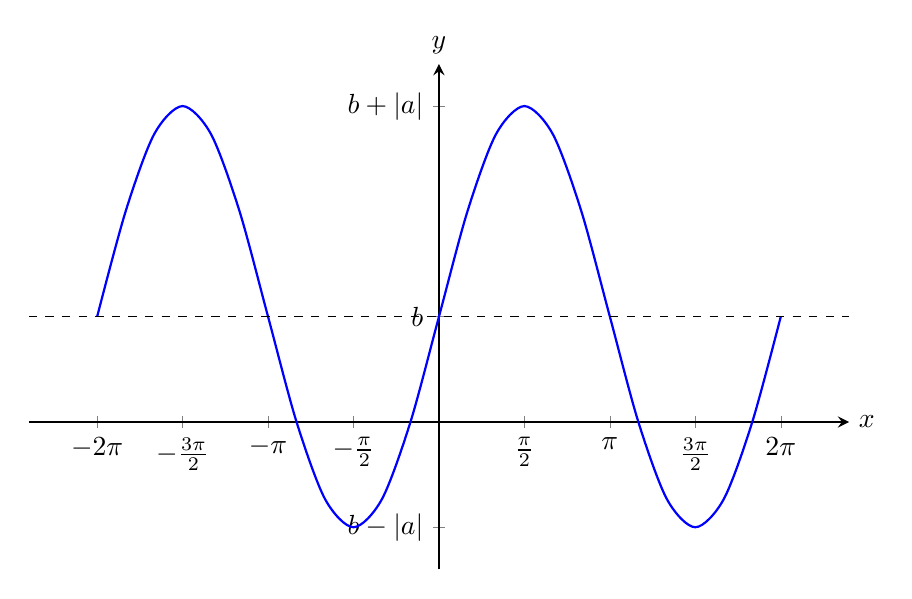
\begin{tikzpicture}
\tikzset{%%
  every mark/.append style={scale=1.0},%%
  scale=1.0%%
}
\pgfplotsset{%%
  every axis/.append style={font=\normalsize}%%
}

\begin{axis}[%%
  axis line style=thick,%%
  axis lines=center,%%
  enlargelimits=true,%%
  height=8cm,%%
  plotStyle/.style={%%
    domain=-2*pi:2*pi,%%
    mark=none,%%
    smooth,%%
    thick%%
  },%%
  width=12cm,%%
  %%
  %% x-axis
  xlabel={\normalsize $x$},%%
  xlabel style={right},%%
  xtick={%%
    -6.283185,-4.712388,-3.141592,-1.570796,%%
    0,%%
    1.570796,3.141592,4.712388,6.283185%%
  },%%
  xticklabels={%%
    $-2\pi$,$-\frac{3\pi}{2}$,$-\pi$,$-\frac{\pi}{2}$,%%
    0,%%
    $\frac{\pi}{2}$,$\pi$,$\frac{3\pi}{2}$,$2\pi$%%
  },%%
  %%
  %% y-axis
  ylabel={\normalsize $y$},%%
  ylabel style=above,%%
  ytick={-1,1,3},%%
  yticklabels={$b-|a|$,$b$,$b+|a|$}%%
]
%%
%%
%% The general sine function f(x) = a sin(x) + b.
\addplot+ [plotStyle]
{2 * sin(deg(x)) + 1};
%%
%%
%% Horizontal line through the number b, which is the midline.
\draw[thin,dashed] (axis cs:\pgfkeysvalueof{/pgfplots/xmin},1) -- (axis cs:\pgfkeysvalueof{/pgfplots/xmax},1);
\end{axis}
\end{tikzpicture}

\end{document}
